\chapter{Methodology}

In Chapter 3, we saw that previous work has produced a variety of approaches to depth estimation and visual odometry, using both data-driven and hand crafted solutions. In this chapter, we propose a novel pipeline that behaves similarly to the pipelines described in Chapter 3, with the key distinction of operating on 4D, as opposed to 2D data. The contributions of previous work focus on the use of monocular and stereo image data, while this chapter focuses on developing a pipeline that employs the full breadth of geometric information in the light field. The first section of this chapter describes the tools and methodologies of acquiring a suitable dataset, while the second part derives the pipeline used for our experiments.

\section{Data Acquisition}

\subsection{Ground Truth Pose Data}

\begin{figure}[h]
    \centering 
    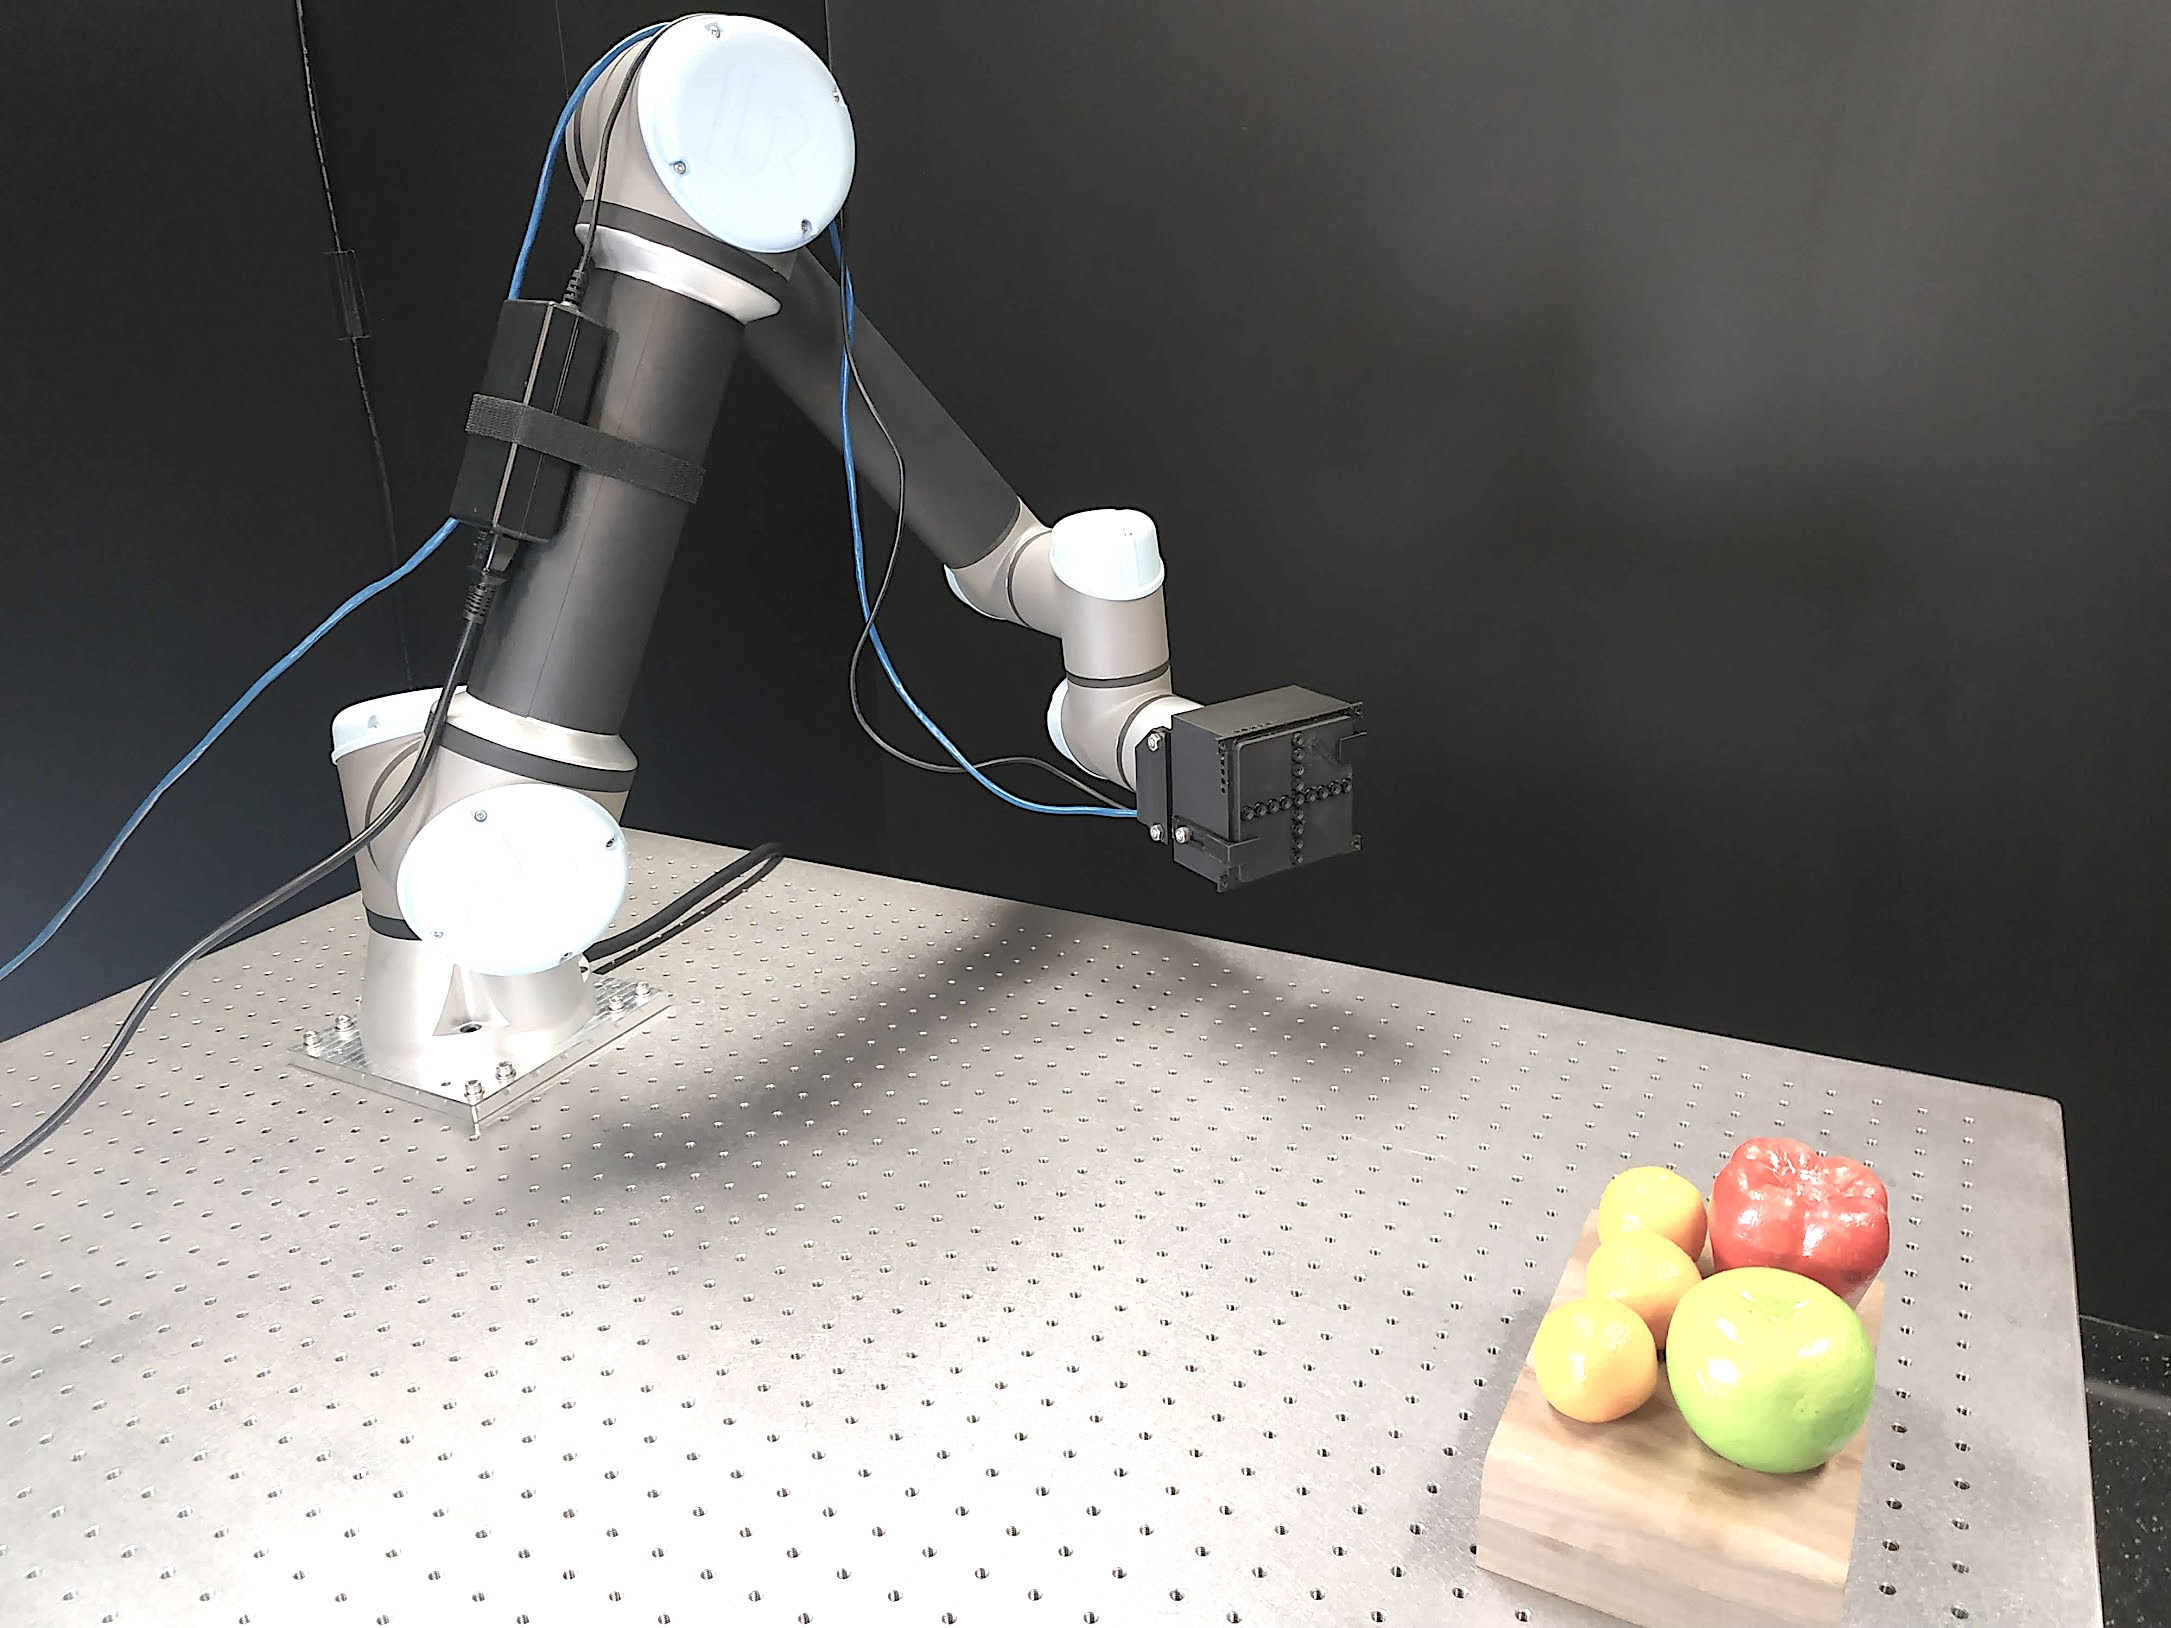
\includegraphics[width=4.5in]{images/experimentalsetup2.jpg}
    \caption[Experimental setup with UR5E manipulator and EpiImaging camera module]{The experimental setup utilises a Universal Robots UR5E robotic arm to precisely measure ground-truth pose to allow effective evaluation of the projects visual odometry results.}
\end{figure}

Important to this work is a strong evaluation framework. Existing datasets such as KITTI and CityScapes benefit from state-of-the-art sensor suites including inertial sensors and lidar, allowing researchers to effectively benchmark their results. Similarly, this thesis places a strong emphasis on validation using ground truth data. One of the primary tasks for evaluation is visual odometry, and so ground-truth pose data for each image is a valuable resource. In this project, pose is collected by attaching the camera to a Universal Robots UR5E robotic manipulator, which is capable of sensing to a high degree of accuracy the pose of the end effector. Furthermore, the UR5E is able to perform accurate movements and trajectories with payloads of up to 5 kilograms, making it a suitable robotic mount for the camera. 

\subsubsection{Manipulator-Camera Interface Adapter}
The UR5E uses a standard interface plate for attaching end-effectors such as gripping tools. The camera on the other hand, despite its excellent construction, is an early prototype provided by EPIImaging, without a physical adapter interface for the UR5E manipulator. We therefore fabricate our own mount for the device, taking into consideration the camera's ventilation and cabling requirements. A two-piece adapter was designed in SolidWorks and fabricated using a fused deposition modelling (FDM) platform with polylactic acid (PLA) filament. 

\subsubsection{Manipulator Control}
A client library for communicating with the UR5E was developed in python, establishing a TCP/IP connection with the robot over the local network, allowing both movement commands to be sent to the robot, and feedback data about the end-effector's pose to be streamed back to the client PC. The client library also provides functionality for computing trajectories and corresponding joint angles, using the PyBullet \cite{pybullet2017} physics engine and the known kinematic model. One useful trajectory function from our library procedurally generates waypoints while keeping the camera's field-of-view trained on the scene, using a stringent collision-checking mechanism to enable autonomous data-capture. 

\subsection{Imagery}
The specific imaging device being used is manufactured by EPIImaging, and consists of 17 sub-apertures. The communication interface with the camera is a network connection serving image data using the HTTP protocol via a REST API. Both rectified and un-rectified imagery can be retrieved, and the format of the returned data is a $17\times 3 \times 1280 \times 960$ stream of raw bytes representing 8-bit pixel values from each of the 17 sensors. A simple client library was developed in python to automate API requests, and perform decoding of the pixel data.

\section{Architectural Overview}
In this section, we derive a pipeline for simultaneous depth and visual odometry using light field data. Our pipeline is constructed modularly, so to build a precise intuition for how our pipeline operates, we begin by providing an architectural overview, followed by detailed descriptions of each individual module. We introduce the CNN modules used to estimate pose and depth. Subsequently we'll discuss strategies for forming meaningful loss-functions to train our pair of networks using a photometric-warp loss-module. Next, we launch a discussion on the input formats, altering how light field data is fed to our networks, discussing the comparable advantages and disadvantages of each. Finally, we introduce some modifications to the photometric-warp loss-module that sacrifices some flexibility in exchange for more robust depth and pose estimates that more-fully exploit information in the light field. 

\subsection{Learning Pipeline Overview}
Like \cite{zhou2017unsupervised}, we exploit the properties of a moving camera - often dubbed `shape-from-motion' - to learn depth and visual odometry in an unsupervised manner. Our learning pipeline is composed of three central modules - depth estimation, pose estimation, and a bilinear interpolation photometric warp module. These three modules work cohesively to estimate a novel view of the scene - i.e. the next frame of video. Using our actual knowledge of what the next frame of video looks like, we compute a fully differentiable loss function which allows the application of a gradient update to the parameters of the depth and pose estimation modules. The architecture is illustrated in Figure 4.2.

\begin{figure}
    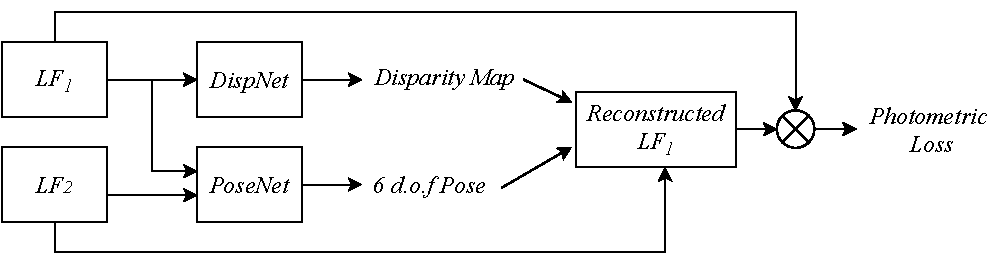
\includegraphics[width=\textwidth]{images/archs/unifiedpipeline.pdf}
    \caption[An architecture for unsupervised learning of depth and pose from light fields]{Our three main modules work together to estimate what the next frame of video looks like. Using our actual knowledge of what that frame looks like, we compute a photometric loss, which is back-propagated and used to apply gradient updates for the disparity and the pose networks.}
\end{figure}

\subsection{Pose Estimation}

We treat pose estimation as a regression problem, estimating three translational components [X, Y, Z] and three rotational components [Rx, Ry, Rz]. We perform this regressions with a convolutional network, which we call `PoseNet', in line with previous work \cite{zhan2018deepfeature,bian2019consistency,zhou2017unsupervised}. This network architecture is fully convolutional, meaning that in principle, it operates on arbitrarily large or small images. 

\begin{table}[h]

    \caption{PoseNet Convolutional Network Architecture}
    \centering
    \begin{tabular}{@{}llllll@{}}
        \toprule
        Layer               & Kernel Size   & Output Channels   & Stride    & Padding   & Activation\\ 
        \midrule
        Conv1               & 7             & 16                & 2         & 3         & ReLU      \\ 
        Conv2               & 5             & 32                & 2         & 2         & ReLU      \\ 
        Conv3               & 3             & 64                & 2         & 1         & ReLU      \\ 
        Conv4               & 3             & 128               & 2         & 1         & ReLU      \\
        Conv5               & 3             & 256               & 2         & 1         & ReLU      \\
        Conv6               & 3             & 256               & 2         & 1         & ReLU      \\
        Conv7               & 3             & 256               & 2         & 1         & ReLU      \\
        Output              & 1             & 1                 & 1         & 1         & -         \\ 
        \bottomrule
    \end{tabular}
    \label{posenet-layers}
\end{table}

\begin{figure}
    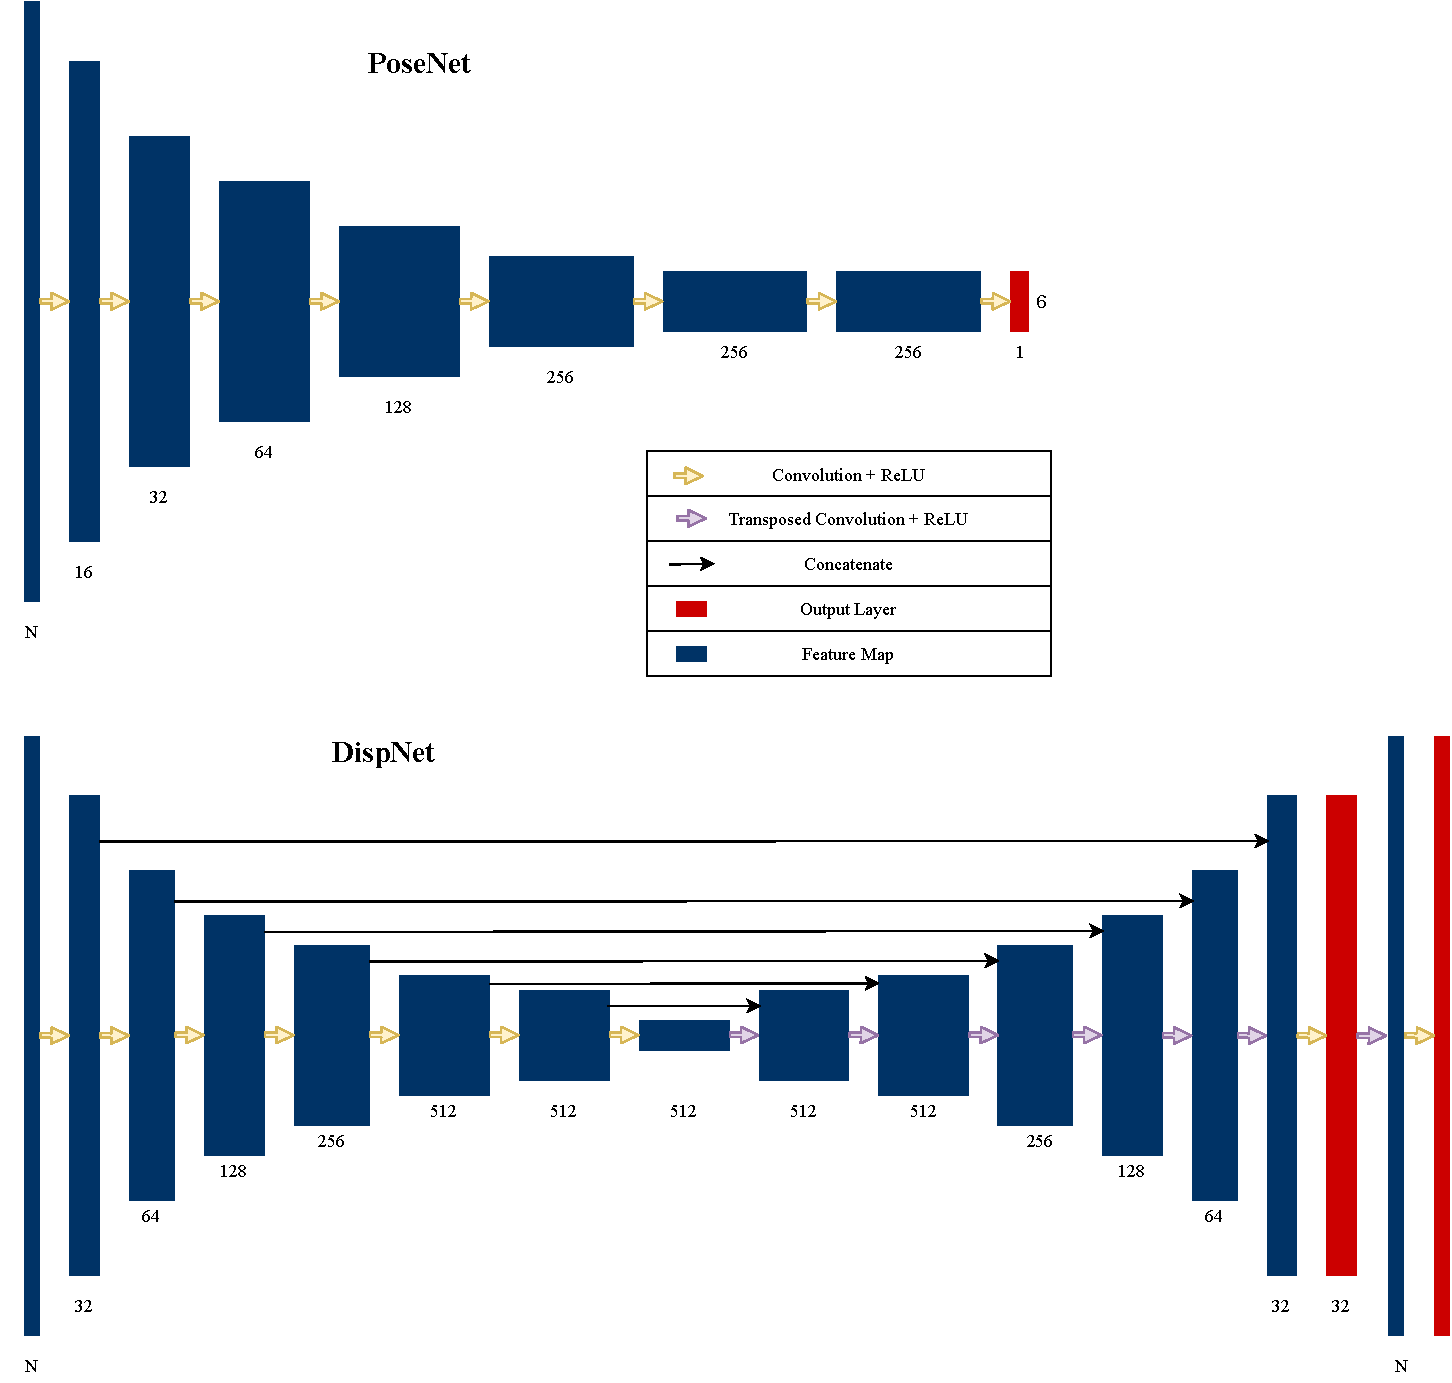
\includegraphics[width=\textwidth]{images/archs/unifiedarch.pdf}
    \caption[The PoseNet and DispNet convolutional architectures]{The PoseNet architecture is a fully convolutional neural network. The input is of shape $H \times W \times N$, and the output shape is $6 \times 1 \times 1$ - one output for each of the 6 degrees of freedom predicted. Similarly, the DispNet architecture is a fully convolutional network that outputs disparity maps at two different scales (shown in red). Skip connections allows the incorporation of both high and low level features in estimating disparity. In the first variant of our algorithm, there is a single output channel, predicting a disparity map aligned with the center view of the camera array. In the second variant, there are $N$ output channels - one for each sub-aperture. These layers are displayed for illustrative purposes only, and are not to scale. }
\end{figure}

% Importantly, the translation and rotation are regressed relative to the \textit{camera} coordinate frame of the first image, whereas the UR5E returns absolute position and orientation in the \textit{world} coordinate frame. To validate our predictions we therefore need to compute the relative translation $P_{t1 \rightarrow t2}$ and rotation $R_{t1 \rightarrow t2}$ of the two images, given their absolute positions $P_{t1}, P_{t2}$ and orientation $R_{t1}, R_{t2}$ in the world frame. Concatenating translation and rotation into a single homogenous transform matrix $T = [R|t]$ allows us compute both relative rotation and translation in a single step, as:

% \begin{equation}
% T_{t1 \rightarrow 2} = T_{t1}^{-1} T_{t2}.
% \end{equation} Intuitively, this computation first computes the transform from pose 1 to the world frame, then from the world frame to pose 2. We can decompose this matrix into 3 translational and 3 rotational components. 


\subsection{Depth Estimation}

Depth estimation is similarly modeled as a regression problem, with two output layers - regressing half- and full-scale depth map predictions. The depth estimation module uses the fully-convolutional encoder-decoder `DispNet' architecture \cite{mayer2015dispnet}. Skip connections from the encoder to the decoder mean the decoding layers are able to access both high level features and low level features on either side of the latent space. Prior work \cite{zhou2017unsupervised} has demonstrated that predicting depth maps at multiple scales improves photometric reconstruction error by enforcing some level of local smoothness. In practice, this helps the network learn to predict depth in challenging, textureless regions of the image. 

\begin{table}[h]

    % \caption{DispNet Convolutional Network Architecture}
    \centering
    \caption{DispNet Convolutional Network Architecture.}
    \begin{tabular}{@{}l|lllllll@{}}

        \toprule
        & Layer       & Kernel Size   & Concatenate   & Output Channels   & Stride    & Padding   & Activation\\ \midrule
        \multirow{7}{*}{\rotatebox{90}{Encoder}}    
        &Conv1       & 7             & -             & 32                & 2         & 3         & ReLU     \\ 
        &Conv2       & 5             & -             & 64                & 2         & 2         & ReLU      \\ 
        &Conv3       & 3             & -             & 128               & 2         & 1         & ReLU      \\ 
        &Conv4       & 3             & -             & 256               & 2         & 1         & ReLU      \\
        &Conv5       & 3             & -             & 512               & 2         & 1         & ReLU      \\
        &Conv6       & 3             & -             & 512               & 2         & 1         & ReLU      \\
        &Conv7       & 3             & -             & 512               & 2         & 1         & ReLU      \\ \midrule
        \multirow{9}{*}{\rotatebox{90}{Decoder}} 
        &UpConv7     & 3             & Conv6         & 512               & 2         & 1         & ReLU      \\
        &UpConv6     & 3             & Conv5         & 512               & 2         & 1         & ReLU      \\
        &UpConv5     & 3             & Conv4         & 256               & 2         & 1         & ReLU      \\
        &UpConv4     & 3             & Conv3         & 128               & 2         & 1         & ReLU      \\
        &UpConv3     & 3             & Conv2         & 64                & 2         & 1         & ReLU      \\
        &UpConv2     & 3             & Conv1         & 32                & 2         & 1         & ReLU      \\
        &Output2     & 3             & -             & 1                 & 1         & 1         & Sigmoid   \\
        &UpConv1     & 3             & -             & 32                & 2         & 1         & ReLU      \\
        &Output1     & 3             & -             & 1                 & 1         & 1         & Sigmoid   \\
        \bottomrule
    \end{tabular}
    
    \vspace{4mm}{}
    \textit{Layers prefixed with `Conv' or `Output' are convolutional layers, and those prefixed with `UpConv' use the transposed-2D-convolution to upsample the preceeding layer.}
    
    \label{dispnet-layers}
\end{table}


\subsection{Photometric Warp Loss}
We have now described one CNN tasked with estimating a per-pixel depth map of the scene, and another which estimates the 6-degree-of-freedom pose between two frames of video. The challenge is now to provide a supervision signal that sufficiently constrains these networks to actually perform the tasks of depth and pose estimation. 

\subsubsection{A Differentiable Loss Function with Image Based Rendering}

As described in Chapter 3, given an estimate for both depth and pose, we can synthesise approximate images of the scene as seen from nearby viewpoints. We take advantage of this fact to form a photometric-warp loss, similar to \cite{zhou2017unsupervised}. 

As described in Chapter 3, the procedure for this is to first project each pixel from the first light field $LF_1$ to a 3D point cloud using the known camera intrinsics and estimated depth values. Recall that the matrix $K$ is the intrinsics matrix introduced in Chapter 2, which maps pixel coordinates to ray directions for a pinhole camera. Using the intrinsics and the regressed depth map $D(s_0, t_0, u, v)$, we can project each pixel $[u, v]^T$ to a 3D point cloud $Q$

\begin{equation}
    Q = D(s_0, t_0, u, v) K^{-1}\begin{bmatrix}u \\ v \\ 1\end{bmatrix}.
\end{equation}
 The 3D coordinate $Q$ is then projected onto the sensor plane of $LF_2$, at the pixel coordinate $[s_0,t_0,\hat{u},\hat{v}]$. This relies on our estimate of the relative pose $[R|t]$ from the first to the second camera origin

\begin{equation}
    [s_0, t_0, \hat{u}, \hat{v}] = K[R|t]Q. 
\end{equation}
The pixels $[s_0, t_0, \hat{u}, \hat{v}]$ are subsequently sampled to populate a new array, forming our synthesised image. This transform is equivalent to constructing a 3D model of the scene using our depth values, moving an imaginary camera by $[R|t]$ and taking a virtual snapshot of the scene from this new angle, the snapshot being the resulting photometric warp. \\

\begin{figure}
    \subfloat[Target Image]{
        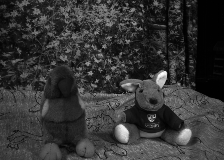
\includegraphics[width=0.24\textwidth]{images/result-examples/warps/seq51/input.png}
    }
    \subfloat[Predicted Depth]{
        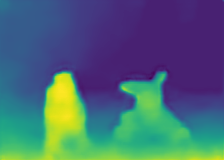
\includegraphics[width=0.24\textwidth]{images/result-examples/depth/multiwarp/epi/51-69.png}
    }
    \subfloat[Synthesised Image]{
        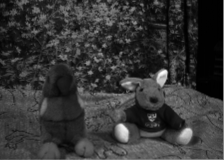
\includegraphics[width=0.24\textwidth]{images/result-examples/warps/seq51/warped.png}
    }
    \subfloat[Photometric Error]{
        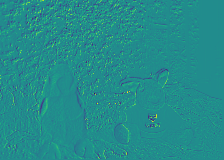
\includegraphics[width=0.24\textwidth]{images/result-examples/warps/seq51/diff.png}
    }

    \caption[The bilinear interpolation algorithm used for differentiable image-based rendering]{To recreate the target image, we use the depth map to calculate the pixel coordinates of the source image from which to sample. The source image is then sampled using bilinear interpolation to reconstruct the synthesised image. The reconstructed and target image are then compared to calculate the photometric error.}
\end{figure}

\begin{figure}
    \centering
    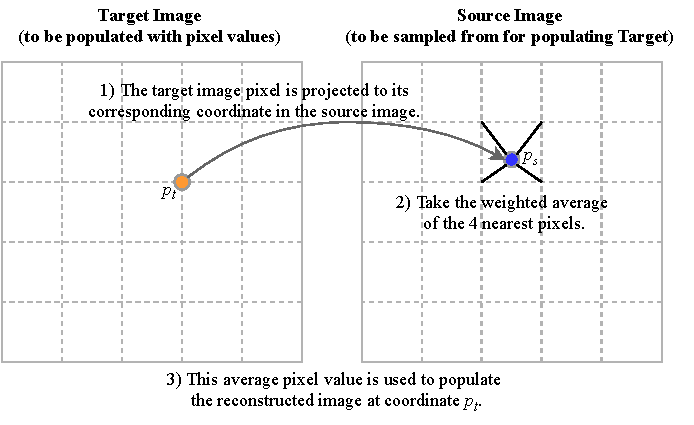
\includegraphics[width=\textwidth]{images/interp.pdf}
    \caption[How bilinear interpolation is used to populate a target image]{We use bilinear interpolation as the differentiable sampling process, just as suggested in \cite{zhou2017unsupervised}. To populate each pixel value $p_t$ in the target image, each pixel is projected to its corresponding coordinate in the source image, and sampled using bilinear interpolation.}
\end{figure}

More broadly, the practice we have described here is referred to as `image based rendering', which is a related, but slightly different paradigm from the rasterization, shaders and textures typically used in geometry-based rendering engines. In image based rendering, we instead synthesise viewpoints using existing image data. In a sense, image based rendering simply shuffles the pixels of an existing image around, according to some pre-defined rules. In our case, we derive the shuffling-rules using 3D data inferred by our depth and pose networks. 

The perceptive reader may have noticed that the pixel value $p_2 = [s_0, t_0, \hat{u}, \hat{v}]$ is continuous in $u$ and $v$, while pixel coordinates are, by necessity, discretely valued. A naive solution is to discretise the coordinate $p_2$ by sampling its nearest-neighbouring pixel. We must remember however that neural networks rely on the chain rule of calculus to perform back-propagation, and so whatever sampling regime we choose must be differentiable. We therefore turn to bilinear sampling, as described in Chapter 3 as a differentiable sampling mechanism. Its operation and derivatives are described in equations 3.3-3.5.

This sampling-based approach is limited in regions surrounding occluders. When the motion of the camera dis-occludes part of the scene in the target image, the sampler is tasked with recreating an image using information that it does not have. Thus, we are most likely to see 3D boundaries as one of the main sources of error. Furthermore, this formation of a loss function assumes a texturally rich image which can be used to compute the error. These effects are apparent in Figure 4.4 (d), where we observe heavy errors around 3D boundaries, as well as texturally rich regions of the image.


\subsection{Input Methods}

This work tackles an interesting and unique challenge, of how to feed sparse light field data to convolutional neural networks. We summarise this challenge as:

\textit{Given sparse 4 dimensional data, how best can we arrange that data as 2 dimensional slices in a valuable and informative way to a convolutional network for the purposes of visual odometry and depth estimation.}

As we have seen in Chapter 3, this problem has been approached in prior work, usually with the assumption that a complete 2D grid of 2D images is available. In this work however, the specific camera configuration prohibits arranging our data as a 2D grid of images without introducing significant redundant data. In a way, this forces us to consider more flexible and generalisable methods for processing light fields into constructive forms of 2 dimensional data. In this section, we suggest three experimental methods for ingesting light field data through neural networks. In the next chapter, we will present visual odometry and depth results using each of these methods.

\subsubsection{Volumetric Images}
The most straightforward of our three methods, this technique involves taking \textit{U, V} slices (perspective-projection images) of the light field, and stacking them along a 3rd axis (usually reserved for the colour-channels). The resulting image is an $H \times W \times N$ volume, where $H$ and $W$ are the height and width of the \textit{U, V} slice, and $N$ is the number of sub-apertures being sampled. This method is suggested, and tested by Wang et al. \cite{wang2016lfcnn} for material classification, who report improved results over conventional 2D imagery. Internally, we expect a convolutional network to learn features relating to parallax, occlusion and depth when exposed to data of this format.

\subsubsection{Focal Stacks}
Focal stacks are constructed as a superposition of 2D images from several sub-apertures, creating interference in regions of the image that are `out-of-focus', while keeping `in-focus' elements of the image crisp. A focal stack specifically encodes depth in the form of interference at each region of the image. Thus, we might expect a CNN trained on this type of imagery to learn to decode in- and out-of-focus parts of the image, using this information to estimate depth and pose. Importantly, we must consider that our spatial sampling rate (distance between sub-apertures) is significantly lower than our angular sampling rate (distance between pixels). As a result our focal stacks exhibit significant aliasing effects which may impact training.

\subsubsection{Tiled Epipolar Plane Images}
In Chapter 3 we saw that Wang et al. \cite{wang2016lfcnn} sliced the 4D light field in two different ways, first as perspective-projection images, and secondly as orthographic-projection images. By showing slices in \textit{S, T} and \textit{U, V}, Wang et al. suggests that a convolutional network is able to learn to approximate 4D signal processing functions without the computational overhead of convolving in 4 dimensions. Due to the specific constraints of the camera array being used (and indeed of any camera array not arranged as a regular grid of sub-apertures), there are challenges associated with slicing our light field data as orthographic images. We suggest that there is indeed another meaningful way of slicing the 4D light field into 2D arrays - namely as epipolar plane images. As we discussed in Chapter 2, epipolar plane images are \textit{S, U} or \textit{T, V} slices of the light field, encoding depth and occlusion in the slope of their characteristic sheared lines. With our input strategy, we tile \textit{T, V} slices side-by-side, and \textit{S, U} slices top-to-bottom. 

\begin{figure}[H]
    \centering
    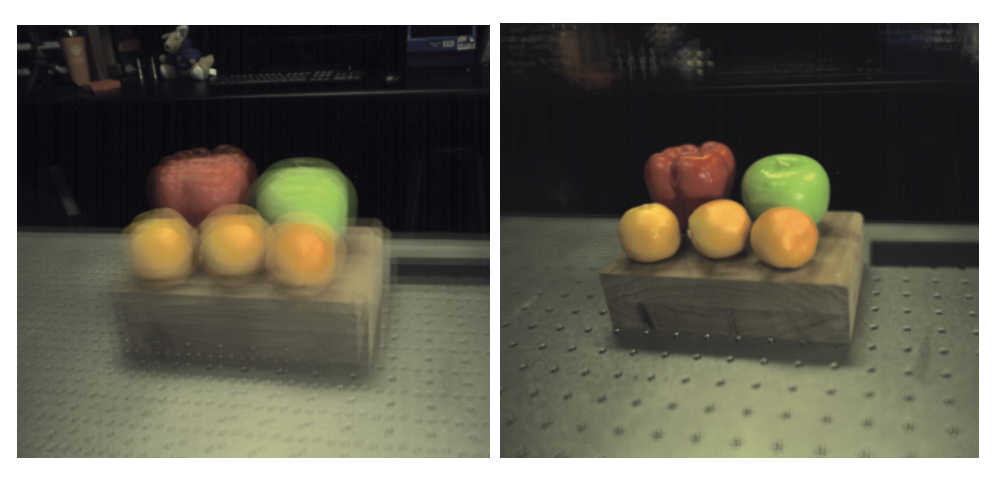
\includegraphics[width=0.7\textwidth]{images/fruitfocus.png}
    \caption[Artifacts from synthetic refocusing]{While synthetically changing the focal plane brings different parts of the scene into focus, the trade-off is the aliasing and artifacts that arise. In this example, we show two synthetically refocussed images, performed using 5 of the 17 available light field samples. The artifacts are especially clear around the boundaries of the fruit shown here - not only are they blurry, but distinct artifacts and ghostlike edges are clearly visible.}
\end{figure}

\begin{figure}[H]
    \centering 
    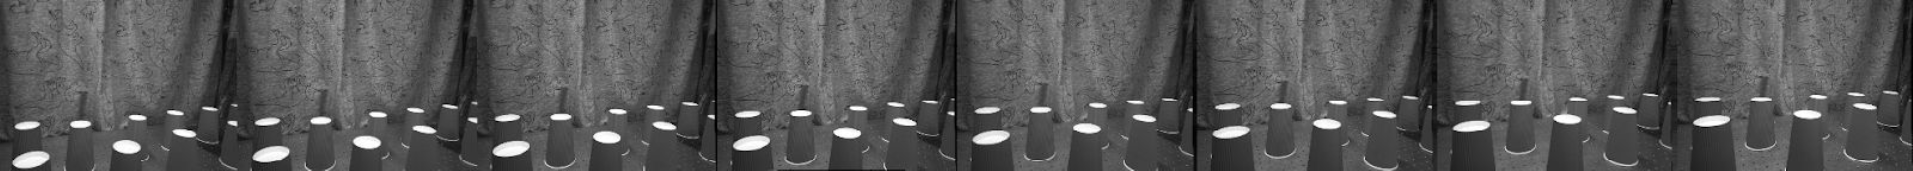
\includegraphics[width=6in]{images/epitile_3.png}
    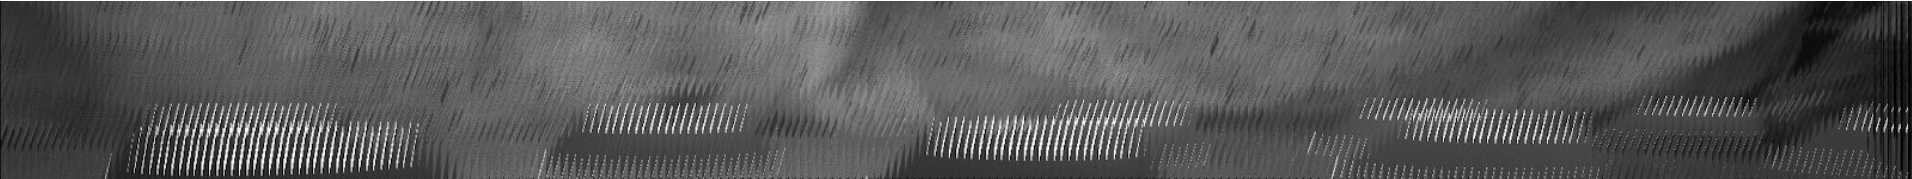
\includegraphics[width=6in]{images/epitile_2.png}
    \caption[Two different ways of slicing the light field]{Tiled \textit{U, V} slices (top): this is an intuitive way of slicing the light field, which tiles images from each sub-aperture side-by-side. Tiled \textit{T, V} slices (bottom): somewhat less intuitively, this method instead tiles the vertical epipolar-plane images side-by-side. We call these \textit{wide} EPIs. As shown, the overall dimensionality and shape of the light field is unchanged, we simply present the information in a different order, revealing different encodings of the captured scene. We can also tile the light field as \textit{S, U} slices, stacking them vertically, which we refer to as \textit{tall} EPIs.}
\end{figure}

\begin{figure}[h]
    \centering 
    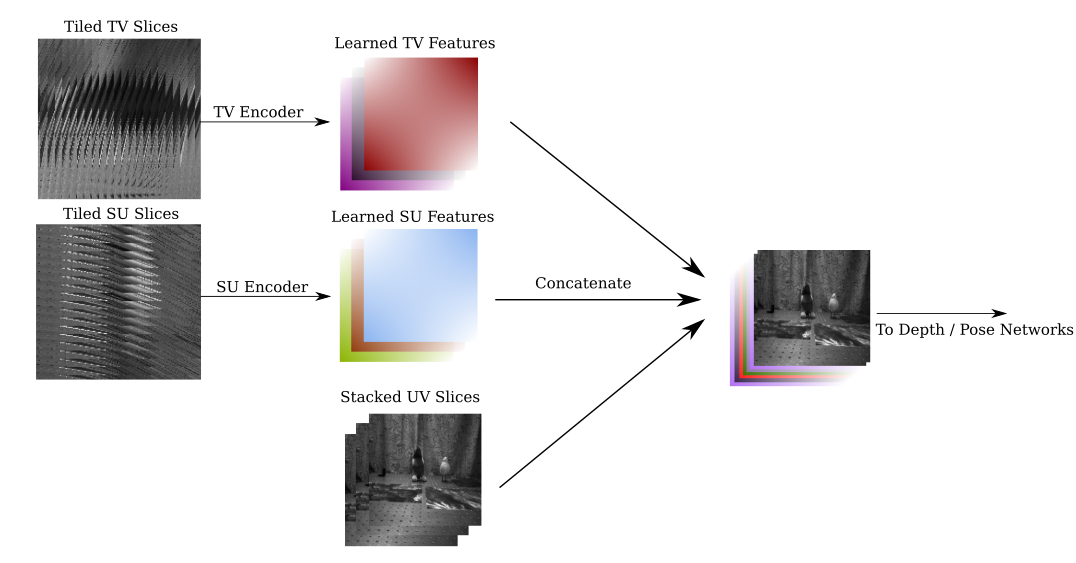
\includegraphics[width=6in]{images/encoderpipe.png}
    \caption[An encoder module for extracting features from EPIs]{Our proposed encoder module which encodes the tiled EPIs, downsampling them to the shape expected by our depth and pose networks. Notably, features which have been learned in \textit{T, V} as well as \textit{S, U} are concatenated with the stacked \textit{U, V} slices (exactly as seen in our first input method.) For brevity, we have only shown a small patch of the tall and wide EPIs, but the reader is reminded that these tilings are in fact very tall, and very wide.}
\end{figure}

\newpage

One challenge we face in ingesting this data, is that both previously described methods have input shapes $H \times W$. The tiled images from Figure 2.4 on the other hand have shape $H \times (W \times N)$ where $N$ is the number of sampled sub-apertures. In practice, these images are much wider than either of our previous input formats. We therefore suggest the use of an additional convolutional encoding module that down-samples the tiled EPIs to the shape expected by our depth and pose networks.

The encoding module consists of one convolutional layer followed by a ReLU activation layer. For the \textit{wide} EPIs we convolve with a kernel of size $N \times N$, and a horizontal stride of $N$. Zero-padding is applied to the top and bottom of the tiled EPI. The effect of this convolution is that the wide EPI is down-sampled with the same output size as a single \textit{U, V} slice. Similarly, we apply an $N \times N$ filter with a vertical stride of $N$ to the tall EPIs, also reducing their shape to that of a \textit{U, V} slice. The resulting feature maps are combined with the \textit{U, V} slices, and provided to our depth and pose networks. Thus, our networks are able to learn features in three different feature spaces. We hypothesise that with this ingestion strategy, our networks are able to learn an approximation for 4D signal processing functions, without the computational overhead of convolving in 4 dimensions, and without the requirement for a complete 2D grid of images.


\subsection{Single-View vs. Light Field Reconstruction}



In this section, we modify our pipeline to more-fully take advantage of the information in the light field. One important weakness of the pipeline we have described so far, is that there are no constraints on our networks to estimate scale with the same magnitude between video frames. Given three frames of video of the same scene, and stable camera motion, the depth network will happily estimate a room that is twice as large in the second pair of frames than the first, if of course the pose network also estimates a twice-as-large translation. This is the scale ambiguity that we have discussed in Chapter 2. With the modifications suggested in this section, we take advantage of the fact that we have multiple sub-apertures capturing the scene at the same time, using this knowledge to enforce scale consistency across video frames. 

The modification described here is straightforward, but it sacrifices some flexibility. The pipeline as we have described it so far requires only one vital piece of information to learn depth and visual odometry - the focal length of the camera being used (assuming all sub-apertures have very similar focal lengths). With this modification, we are required to at least know the arrangement of the sub-apertures in relation to one-another (although the absolute scale of their layout is not required). In our case, we know that our sub-apertures are arranged as a cross-hair. 

\begin{figure}[htbp]
    \centering 
    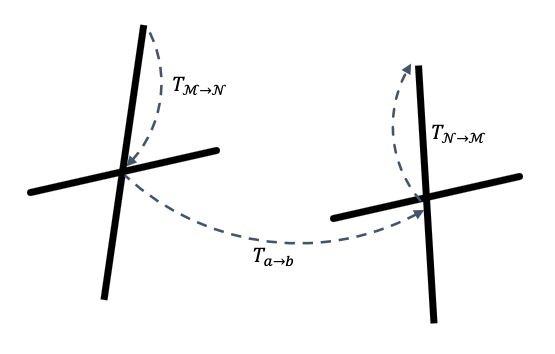
\includegraphics[width=3.5in]{images/relative_subapertures.png}
    \caption[The relationship between sub-apertures as the light field camera moves through space]{Given knowledge of how one sub-aperture has moved through space, we can also compute how any other sub-aperture has moved by chaining the transforms in the order shown.}
\end{figure}

Instead of using photometric warp to reconstruct the image of a single sub-aperture, this modification adjusts the pipeline such that instead, we now reconstruct the entire light field. The camera array is a rigid body, meaning that as it rotates and translates through space, the sub-apertures also rotate and translate relative to each other, but in a very well defined way. Say we know the homogenous transform  $T_{a \rightarrow b}$ of sub-aperture $\mathcal{N}$ between two frames of video, we can compute the global transform of any other sub-aperture $\mathcal{M}$ by chaining together the homogenous transforms as shown in Figure 4.9.

To exploit this knowledge, we modify the depth prediction network to now output $N$ depth maps. Each depth map should be aligned with exactly one sub-aperture, so we can reconstruct its corresponding image. The pose network continues to estimate only the pose of the central sub-aperture, but the frame-to-frame pose for each pinhole is computed from the chained transform shown in Figure 4.9 (where $T_{a\rightarrow b}$ is the PoseNet output). For each sub-aperture we perform the same photometric warp with bilinear interpolation to synthesise $N$ viewpoints.

In addition to imposing a stronger supervision signal, this pipeline guarantees to a certain extent that our pose and depth modules predict depth at a consistent scale between video frames. We have enforced a photometric warp that requires prior knowledge of the shape of the camera, and with this information now making up a part of the photometric-warp pipeline, our neural networks are forced to learn to use this information to estimate depth and pose at the correct scale. To see why this is true, we should consider the effect on the loss function for an incorrectly estimated scale-factor. We may find that estimating a twice-as-large room for a twice-as-large translation works to photometrically warp the center-view well, but this will be disastrous for each of the other $N-1$ sub-apertures being warped. In short, our networks are penalised harshly for incorrect scale estimates.
